\graphicspath{{Appendix/appendix_0d-mirror/}}

%\newcommand{\phil}[1]{\marker{cyan}{phil}{#1}}  % Phil
\newcommand{\kunal}[1]{\marker{green}{Kunal}{#1}}  % Kunal
\newcommand{\bad}[1]{\marker{red}{problem}{#1}} 
%\newcommand{\todo}[1]{\marker{purple}{To do}{#1}} 

\chapter{0D mirror optimization}
\label{app:0d-mirror}

%\begin{enumerate}
%    \item \bad{Main things that need to be done: find references and double check the equations}
%    \item \bad{Power to central cell isn't accounted for in plug temperature caluations — fudge factor is used}
%\end{enumerate}
%
%\begin{enumerate}
%    \item \todo{Check that DT alpha orbit is contained}
%    \item \todo{Add HHFW heating to increase Einj above Ebeam}
%    \item \todo{Add neutron dpa}
%    \item \todo{Implement assumption calculations for FLR effects and the paraxial approximation}
%    \item \todo{Add FLR stabilization estimate (Eq 38 in "Magneto-hydrodynamically stable[...]", Ryutov 2011}
%    \item \todo{Add neutral beam shine through as a condition for plasma density}
%    \item \todo{Compare to baseline in section 7 of Egedal et al 2022 \cite{Egedal_2022}}
%    \item \todo{Implement beta-enhanced mirror ratio limits from diamagnetic-bubble paper. Beta-enhanced mirror ratio flag?}
%    \item \todo{Add "tail wagging" stabilization power cost}
%    \item \todo{Calculate stability thresholds and growth rates}
%\end{enumerate}

%\tableofcontents
%\listoffigures
%\listoftables
%\newpage

This appendix describes a 0d mirror reactor optimization project. The equations and assumptions used for this optimization are described. This project provided good intuition on the limitations of simple mirrors. In addition, it gave practical experience using SymPy and Jax. The work has yet to be extended to tandem mirrors.

This work was built off an Excel spreadsheet created by Cary Forest, with contributions from Kunal Sanwalka.

\section{List of assumptions / conditions}

There are many issues and assumptions with this analysis (in no particular order):
\begin{enumerate}
    \item Powers and particles are not strictly balanced in tandem mirrors
    \item Thermal barriers are ignored which may be very important for a practical reactor
    \item A fudge factor is used for electron temperatures when plug electrons are heating the central cell
    \item Macrostability is not considered
    \item Microstability is not considered
    \item Plug confinement time is not self-consistent with plug temperatures
    \item Effects of field ripple are not calculated
    \item T-T and T-He3 reaction rates are not considered
    \item Radial transport is assumed to be only classical 
    \item Cat-DD assumes instant burnup of products which is unreasonable, particularly at the high ion energies needed in mirror reactors
    \item Impurities are assumed to be zero
    \item Heating and magnet costs are not justified 
    \item All fusion power exits the plasma immediately (charged particles are collected by the direct-energy converter, neutrons absorbed by the blanket)
    \item When using the temperature model from Egedal 2022 \cite{Egedal_2022}, we assume that the auxiliary power is much less than the beam power ($P_{aux} / P_{NBI} \ll 1)$ or else the model may be inaccurate. Auxilary power (say, to compensate for classical diffusion losses or additional ECH) can be included in this model but it would require interative solving.
    \item Burnup fraction is sufficiently small that fusion reactions are not a significant loss of fuel (ironically).
    \item The DECs collect all ion losses at a fixed efficiency
\end{enumerate}

\section{User specified parameters}

\subsection{Simple mirror endplug}

\begin{enumerate}
    \item Mirror field, plug (T): $B_{p, m}$
    \item Plug (i.e., midplane) cell field (T): $B_p$
    \item Magnet bore/throat radius (m): $r_b$
    \item Plug length (m): $L_p$
    \item Neutral beam energy (keV): $E_{\text{inj}}$ or $E_b$
    \item Beta limit (critical stability): $\beta_{limit}$ (set to 0.8 \cite{KOTELNIKOV_2021})
    \item Effective species mass (amu): $\mu$
    \item Effective atomic number (account for He and other impurities): $Z_{\text{eff}}$
\end{enumerate}

The $\beta_{limit}$ (discussed in Kotelnikov 2021 \cite{KOTELNIKOV_2021}) assumes a stationary plasma (no rotation, no flow out the ends), ignores finite-Larmor-radius (FLR) effects (which stabilize $m > a^2/L \rho_i$ modes), and uses the paraxial approximation ($L_m \gg a$). It also assumes $\beta \ll 1$ but this paper shows that these results match up with GDT experiments. The $\beta_{limit}$ depends on the radial pressure profile falloff; the faster the falloff, the lower the $\beta_{limit}$. $L$ is the length from midplane to throat, and $L_m$ is the length of the mirror (highest field to lowest, I think). Profile calculations will not be included in a 0D optimization. The relevant assumptions for FLR effects and the paraxial approximation should be calculated and shown in the output to make sure they are not dramatically violated.

\subsection{Tandem mirror}

Central cell parameters defined below. Simple mirror endplugs are used on either end.

\begin{enumerate}
    \item Central cell field (T): $B_{cc}$
    \item Central cell to plug density ratio: $n_{\textit{cc}}/n_p$
    \item Central cell ion to plug electron temperature ratio: $T_{\textit{cc,i}}/T_\textit{p,e}$ (assumes Maxwellian)
    \item Central cell to plug electron temperature ratio: $T_{\textit{cc,e}}/T_\textit{p,e}$
    \item Central cell length (m): $L_{cc}$
    \item Electron temperature fudge factor: $T_{\text{ep, fudge}}$ if electron are heating the central cell. Default value is 0.5
\end{enumerate}

\subsection{Engineering parameters}

\begin{enumerate}
    \item Vessel wall radius (with respect to plasma radius): $a_{\text{wall}} = a_\text{wall, ratio} \cdot a_\text{plasma}$
    \item Blanket thickness: $d_\text{blanket}$
    \item Vacuum vessel thickness: $d_\text{vv}$
    \item Direct Converter Efficiency (used in the mirror exhaust): $\eta_{DEC}$
    \item Thermal to electric conversion efficiency: $\eta_{TE}$
    % \item Heating System Efficiency (may vary by heating scheme (NBI vs. ICRH vs. ECRH)): $\eta_{HS}$
    \item ECH heating efficiency: $\eta_{ECH}$
    \item NBI heating efficiency: $\eta_{NBI}$
    \item RF heating efficiency: $\eta_{RF}$    
\end{enumerate}

Optimizing the blanket and vacuum vessel thickness would probably require some neutronics calculations which would probably depend on the fuel mix, so we're just going to leave those constant in our optimization.

\section{Fusion}
DT fusion helium energy (keV): $E_\alpha = 3500$

\subsection{Reactivity}
DD and DT fusion cross-section parameterizations can be found in Bosch 1992. \cite{Bosch_1992}. What we care most about is the fusion reaction rate per unit volume (eq. 10 in the paper):
\begin{equation}
    \frac{dR}{dV} = \frac{n_i n_j}{1+\delta_{ij}} \langle \sigma v \rangle
\end{equation}
This parameterization accepts ion temperature in keV and gives reactivity in cm$^3$/s:
\begin{align}
    & \langle \sigma v \rangle = C1 \cdot \theta \sqrt{\xi / (m_r c^2 T^3)} e^{-3 \xi} \\
    & \theta = T \mathbin{/} \left[ 1 - \frac{T(C2 + T(C4 + TC6))}{1 + T(C3 + T(C5 + TC7))} \right] \\
    & \xi = \left( B_G^2 / 4\theta \right)^{1/3} \\
    & B_G = \pi \alpha Z_1 Z_2 \sqrt{2 m_r c^2}
\end{align}
where $m_r$ is the reduced mass and $\alpha$ is the fine structure constant. The coefficients ($C1$, $C2$, and so on) are in the paper cited above. This parameterization is valid for $T_i$ between $0.2$ to $100$ keV. 
%\bad{We will definitely exceed this in our optimization -- the extent of the deviation should be quantified. The cross section explodes for DD after roughly 500 keV}
Max error is 0.25\% for DT and 0.35\% and 0.3\% for DD $\Rightarrow$ p T and DD $\Rightarrow$ n He3, respectively. 
%\phil{We will want to use the cross-section (the parameterization of which goes up to 550 keV for DT in \cite{Bosch_1992}) and integrate over ion distribution. Integration over non-Maxwellian ion distributions should be doable if FBIS \cite{Egedal_2022} can give the full distribution.} \phil{For now I'm just linearly interpolating (in log-log space) between the points provided in the NRL. Comparison plots of the different methods for DD and DT can be seen in figures \ref{fig:DT_reac} and \ref{fig:DD_reac}.}

\begin{figure}
    \centering
    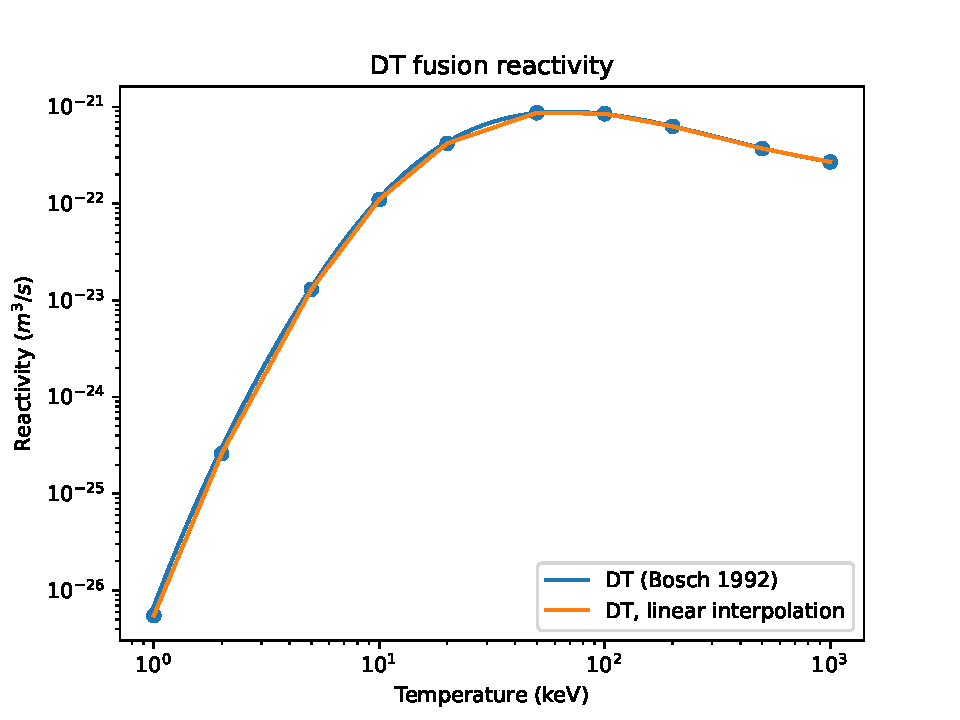
\includegraphics[scale=0.7]{equation_figures/DT_reactivity.pdf}
    \caption{DT reactivities}
    \label{fig:DT_reac}
\end{figure}

\begin{figure}
    \centering
    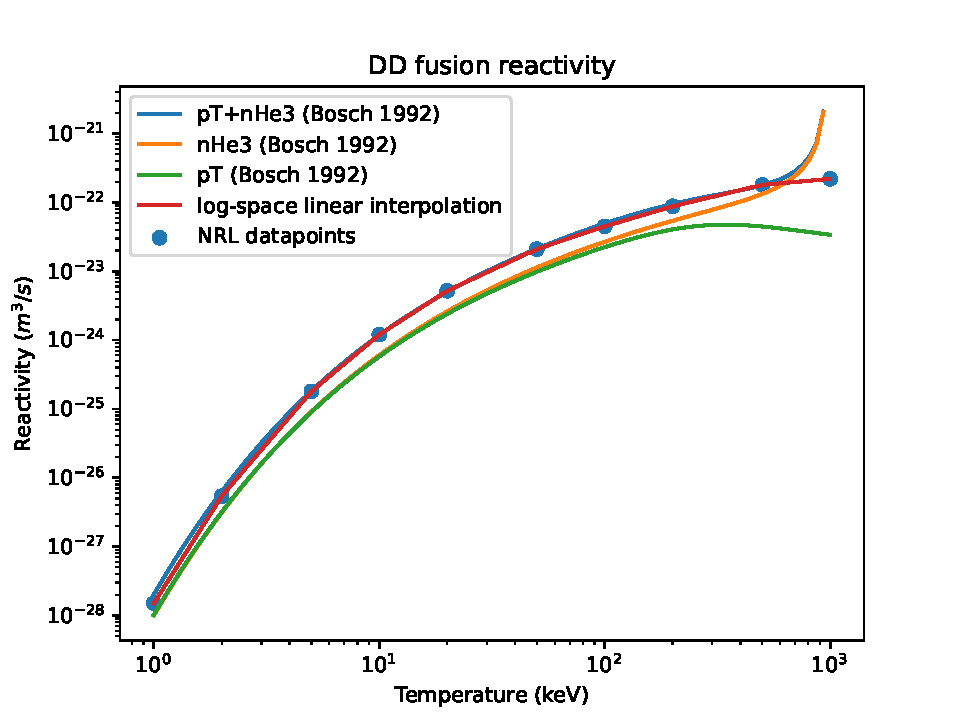
\includegraphics[scale=0.7]{equation_figures/DD_reactivity.pdf}
    \caption{DD reactivities}
    \label{fig:DD_reac}
\end{figure}

\begin{figure}
    \centering
    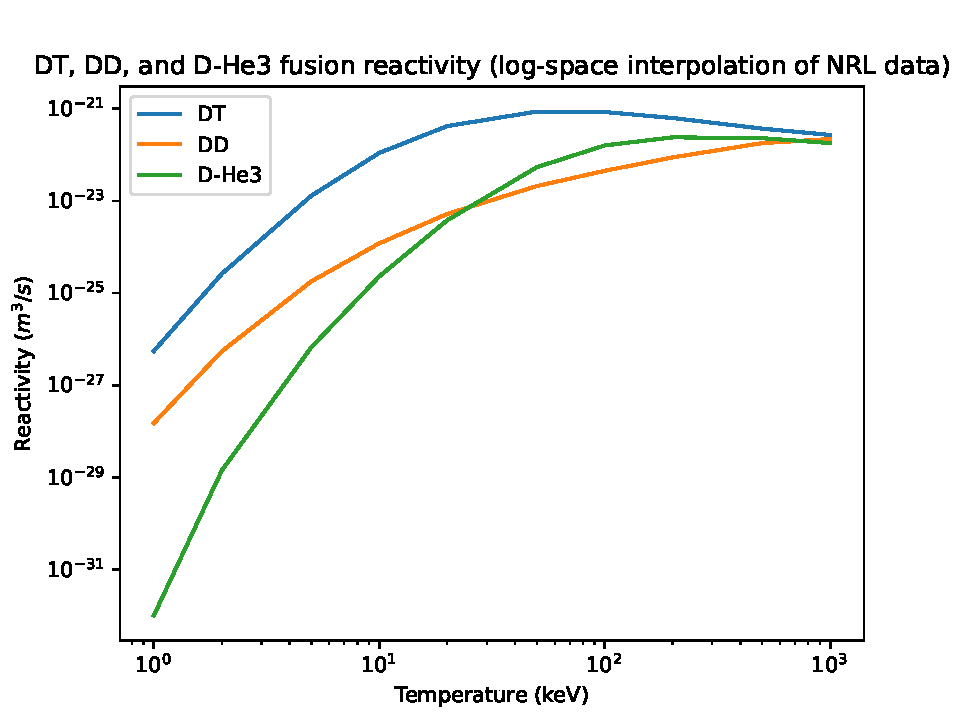
\includegraphics[scale=0.7]{equation_figures/compare_reactivity.pdf}
    \caption{DT, DD, and D-He3 reactivity comparison}
    \label{fig:compare_reac}
\end{figure}

\subsection{Fusion power}

DT fusion reaction rate (\#/s):
\begin{equation}
    R_{\text{x,DT}}= V n_{\text{D}} n_{\text{T}} \langle\sigma v\rangle_{DT}
\end{equation}
If $n_\text{D} = n_\text{T} = n/2$, then this becomes $V \frac{n^2}{4} \langle\sigma v\rangle_{DT}$

DD fusion reaction rate (\#/s):
\begin{equation}
    R_{\text{x,DD}}=V \frac{n_{\text{plug, D}}^2}{2} \langle\sigma v\rangle_{DD}
\end{equation}
The $\frac{1}{2}$ factor is to avoid double counting DD reactions. 

Fusion power (MW):
\begin{alignat}{2}
    &P_{\text{DT,n}} &&= 14.1 |e| R_{\text{x,DT}} \\
    &P_{\text{DT,+}} &&= 3.5 |e| R_{\text{x,DT}} \\
    &P_{\text{DD,n}} &&= 2.45 |e| R_{\text{x,DD}} \cdot \frac{1}{2} \\
    &P_{\text{DD,+}} &&= \left(4.02+0.82 \right) |e| R_{\text{x,DD}} \cdot \frac{1}{2} \\
\end{alignat}
It's useful to split the power into charged and neutrons because energy is extract from them in different ways. Neutrons provide thermal power, charged particles heat the plasma and/or are directly captured by the DECs. The $\frac{1}{2}$ coefficient on the DD reactions assumes a 50-50 split on the DD branching ratio which actually varies with energy and may be significant above around 100 keV. If we assume the tritium produced from a DD reaction is burned instantly, then the additional power produced ("catalyed DD") is:
\begin{alignat}{2}
    &P_{\text{cat DD,n}} &&= 14.1|e| R_{\text{x,DD}} \cdot \frac{1}{2} \\
    &P_{\text{cat DD,+}} &&= \left(3.5+18.3 \right) |e| R_{\text{x,DD}} \cdot \frac{1}{2} \\
\end{alignat}
We assume the tritium is burned instantly because the DT reaction rate is much higher than DD and D-He3 fusion up to around 200 keV, after which it's only slightly higher up to around 1 MeV. A more accurate estimate of fusion power would require estimates of D-He3, TT, and T-He reaction rates and density evolution of each species. A plot of reactivities can be found in Fig. \ref{fig:compare_reac}. 
%\phil{I do not know how to do this steady-state calculation in a simple 0d way -- perhaps this sort of calculation is left for a more detailed reactor model.}

\section{General formulae}

Electron cyclotron frequency (GHz):
\begin{equation}
    f_{\text{ECH}} = \frac{e B}{2 \pi m_e c} = 28 B
\end{equation}

Ion cyclotron frequency (MHz):
\begin{align}
    f_{ci} &= \frac{Z e B}{2 \pi m_i c} \\
    f_{ci, D} &= 7.63 B \\
    f_{ci, T} &= 5.09 B
\end{align}
Here, $Z$ is the charge state of the ion.

Electron plasma frequency (Hz):
\begin{equation}
    f_{pe} = \frac{1}{2 \pi} \sqrt{\frac{4\pi n_e e^2}{m_e}} = 8.98 \cdot 10^3\sqrt{n_{\text{plug}}}
\end{equation}

Ion plasma frequency (Hz):
\begin{align}
    f_{pi} &= \frac{1}{2\pi}\sqrt{\frac{4\pi n_i Z^2 e^2}{\mu m_p}} \\
    f_{pi,D} &= 2100 \sqrt{\frac{n_{\text{plug}}}{2}} \\
    f_{pi,T} &= 2100 \sqrt{\frac{n_{\text{plug}}}{3}}
\end{align}
Here, $\mu$ is the mass of the ion in proton mass units (e.g. $\mu_{\text{Deuterium}}=2$ and $\mu_{\text{Tritium}}=3$).

Lorentz factor ($\gamma$):
\begin{equation}
    \gamma = \sqrt{1+ \frac{T_e}{m_e c^2}} = \sqrt{1 + \frac{T_e}{511 \text{keV}}}
\end{equation}

Ion thermal velocity:
\begin{equation}
    v_{Ti}=97900\sqrt{\frac{10^3E_{\text{ion}}}{\mu}}
\end{equation}

Ion gyroradius: 
%\bad{Cary's spreadsheet uses the temperature to calculate this but calls it "$E_{\text{ion}}$". I think temperature should be used to accurately account for the energy in vperp}
\begin{equation}
    \rho_i = \frac{m v_\perp}{q B} = 3.22\cdot 10^{-3} \frac{\sqrt{\mu E_{\text{ion}}}}{B_p}
\end{equation}

Whistler wavelength:
\begin{align}
    \lambda_{\text{whistler}} &= \sqrt{\frac{2\pi\Omega_e c^2}{\Pi_e^2 f}} \\
    \lambda_{\text{whistler}} &= \sqrt{\frac{90 f_{\text{ECH}}}{f_{pe}^2 f_{D,\text{2nd Harmonic}}}}
\end{align}
The 2nd formula is what appears on the spreadsheet and is used to estimate the size of the RF wave used for HHFW as compared to the size of the plasma. It takes into account the various constants and units used in the spreadsheet.

Collision rates (from NRL):
\begin{align}
    \nu_e &= 2.91\cdot10^{-6}\frac{n_e \ln\Lambda}{T_e^{3/2}} \\
    \nu_i &= 4.80\cdot10^{-8}\frac{Z_{\text{eff}}^4n_i\ln\Lambda}{\mu^{1/2}T_i^{3/2}}
\end{align}

These can be rearranged to give the following collision times (s): 
%\bad{this seems to assume $\log{\Lambda} = 20$ (should be doubled check but doesn't probably make much of a difference -- comparing to eq 4.8 in \cite{baldwin_end-loss_1977}).} \bad{Depends on Zeff which isn't accounted for during optimization/power balance.} \phil{Technically we should use $T = \frac{2}{3} E_{ion}$ for the central cell since the distribution is likely approximately Maxwellian, but it only changes $\tau_{ii}$ by a factor of 1.8.} 
\begin{align}
    \tau_{ee} &= 10^{-4} \frac{T_e^{3/2}}{n_{20} \lambda_{ee}} \\
    \tau_{ii} &= 1.25\cdot10^{-4} \frac{\mu^{1/2} E_{\text{ion}}^{3/2}}{n_{20}Z_{\text{eff}}^4}
\end{align}

Slowing down times \cite{dolan_1982} 
%\phil{I assume Z is Zeff? Need to double check. I put it as Zeff in the ipynb}:
\begin{align}
    \tau_{i,\text{slow}} &= 0.1 \frac{\mu T_e^{3/2}}{n_{20} Z^2 \lambda_{ei}} \\
    \tau_{i,\text{fast}} &= \left( \left( \tau_{ii} 0.4 \log{\frac{R_m}{\sqrt{1-\beta}}} \right)^{-1} + \frac{1}{\tau_{\text{slow}}} \right)^{-1}
\end{align}
Here, we can write $Z=2$ for alpha particles. The 2nd equation comes from substituting the expression for $T_e$ in a purely NBI heated case seen above.

Coulomb logarithms:
\begin{align}
    \lambda_{ee} &= 23.5 - 0.5\ln{n_e} + 1.25\ln{T_{e}} - \left( 10^{-5} + \frac{\left( \ln{T_{e}} - 2 \right)^2}{16} \right)^{1/2} \\
    \lambda_{ei} &= 24 - 0.5\ln{n_e} + \ln{T_e} \\
    \lambda_{ii, \text{Cary}} &= 31 - 0.5 \ln{n_e} + \ln{T_e} \\
    \lambda_{ii, \text{NRL}} &= 23 - 0.5 \ln{n_e} + 1.5 \ln{T_i}
\end{align}
The formula for $\lambda_{ee}$ is from NRL. 
The formula for $\lambda_{ei}$ is from NRL. However, the plasma does not fit into any of the 3 limiting cases described in the formulary. We have picked the formula based on the condition that is violated the least severely. 
There are 2 formulas for $\lambda_{ii}$. They do not have a large disagreement in the ranges of $T_e$ and $T_i$ of interest.

\section{Radial particle transport}

As of the time of writing, diffusive radial transport in mirror reactors appears to be an open question. The goal here is to provide reasonable estimates of radial particle loss and how each scale, not necessarily going for high-accuracy predictions (though being close would be nice!)

\subsection{Classical diffusion}
Assuming Fick's law and a linear density gradient from 3n to 0 (from Chen 5.8): 
\begin{equation}
    \tau_\text{classical} = \frac{n V}{A \cdot \Gamma} = \frac{n a}{-2 D_\perp \nabla n}
\end{equation}
where $D_\perp$ is defined as 
\begin{equation}
    D_\perp = \eta_\perp n \sum T / B^2
\end{equation}
and the parallel and perpendicular conductivites are
\begin{align}
    \eta_{||} &= 5.2 \cdot 10^{-5} \frac{Z ln \Lambda}{T^{3/2}} \\
    \eta_{\perp} &= 2 \cdot \eta_{||}
\end{align}
Combining all of this together gives
\begin{equation}
    \tau_\text{classical} = \frac{a^2 B^2 T_e^{\frac{3}{2}}}{3.12 \cdot 10^{-4} \cdot n Z \sqrt{\mu} \ln{\Lambda} \sum{T}}
\end{equation}

\subsection{Bohm diffusion}
%\phil{I don't like how pessimistic the estimates are for this are. Reasonable values gets you 500 $\mu$s confinement times for Bohm diffusion.}
Bohm diffusivity:
\begin{equation}
    D_\text{Bohm} = \frac{1}{16} \cdot \frac{T_{i,cc} \cdot 10^3}{B_{cc}}
\end{equation}

Normalized gyroradius (assuming deuterium):
\begin{align}
    & r_\text{Larmor} = \frac{\sqrt{2 m E_\perp}}{2eB_{cc}} = \frac{0.00791 \sqrt{T_{i,cc}}}{B_{cc}}\text{cm} \\
    & \rho^* = \frac{r_\text{Larmor}}{a_{cc}}
\end{align}

Again, using Fick's law and assuming a linear density gradient from $3 n$ to 0 (so that total particle number remains $n \cdot V$), cross-field particle flux is:
\begin{align}
    \Gamma &= - D_\text{Bohm} \cdot \nabla n_e \\
    & = \frac{1}{16} \cdot \frac{T_{i,cc} \cdot 10^3}{B_{cc}} \cdot 3 n_i
\end{align}
which implies a characteristic confinement time of
\begin{align}
    \tau_\text{Bohm} &= N_\text{tot} \bigg/ \frac{dN}{dt} = n_i \cdot V / \left(\Gamma * A\right) \\
    &= n_i \cdot \pi a^2 L \bigg/ \left(\frac{1}{16} \cdot \frac{T_{i,cc} \cdot 10^3}{B_{cc}} \cdot 3 n_i \cdot 2 \pi a_{cc} L\right) \\
    &= \frac{8 a B_{cc}}{3 T_{i,cc} 10^3}
\end{align}

\subsection{Gyro-Bohm diffusion}

The gyro-Bohm scaling assumes cross-field transport is dominated by small ion-gyroscale turbulence. Though commonly used for tokamak scaling laws, we should be able to get some rough estimates for mirrors. Right now it can be estimated by just diving the Bohm confinement time by the normalized gyroradius $\rho^*$.
The gyro-Bohm estimate is then:
\begin{equation}
    \tau_\text{gyro-Bohm} = \frac{8 a B_{cc}}{3 T_{i,cc} 10^3} \cdot \frac{1}{\rho^*}
\end{equation}
The $\frac{1}{\rho^*}$ factor can boost the confinement time estimate by a factor of 50-100. 
%\phil{But the confinement times still seems a little low.}

\subsection{ETG-driven transport}

%Cary's spreadsheet says 
%\phil{(I'm having trouble finding a derivation or hand-wavy justification)}:
\begin{equation}
    \chi_\text{ETG} = 0.1 \frac{T_{e,cc}^{3/2}}{B_{cc}}
\end{equation}
\begin{equation}
    \tau_\text{ETG} = \frac{a_{cc}^2}{\chi_\text{ETG}}
\end{equation}

\section{Mirror-specific derived quantities}

\subsection{Temperatures and confinement time in a beam-heated mirror from Egedal et al 2022 \cite{Egedal_2022}}

Electron and ion temperature (keV) via pure beam heating \cite{Egedal_2022}: we must solve a system of equations which considers the power balance of the machine. The ion temperature, given by eq. 22 in \cite{Egedal_2022} is:
\begin{align}
    \frac{3}{2} \frac{T_i}{E_{beam}} = \frac{\exp{(-\alpha)} - \alpha \Gamma(0, \alpha)}{\Gamma(0, \alpha)}
\end{align}
Note that eq. 22 in \cite{Egedal_2022} is missing a factor of $\alpha$ in the numerator in front of the $\Gamma$ function. The electron temperature can be found in terms of $T_i$ and $\alpha$ by rearranging the definition of $\alpha$ (eq 21):
\begin{align}
    % \alpha \approx 22.4 \frac{(T_e / E_{beam})^{3/2}}{(T_i/E_{beam})^{1/2} \ln{R_m}}
    \frac{T_e}{E_{beam}} =  \left( \frac{T_i}{E_{beam}} \frac{2}{3} \frac{\alpha^2 \ln{R_m}^2}{(22.4)^2} \right)^{1/3}
\end{align}
These can be solved for with the help of a power (really energy-per-particle) balance equation (eq. 24 in \cite{Egedal_2022}):
\begin{align}
    E_{beam} + p_{aux} = T_i + 6T_e
\end{align}
where $p_{aux}$ is the combined sources and losses, such as alpha-particle heating, plasma heat losses, RF heating, radial transport, and so on. By balancing the power lost with auxiliary heating power we can keep $p_{aux} = 0$ to avoid iteratively solving this equation. Each ion loses $T_i + e \Phi \approx T_i + 5 T_e$ units of energy and each electron loses $\approx T_e$ units because only hotter electrons can surmount the ambipolar potential. $p_{aux}$ isn't so much a power as it is the energy gained/lost per particle -- an actual power would require evaluation of the confinement time (eq 29 in \cite{Egedal_2022}):
\begin{align}
    \tau_p = \tau^{90}_{Ti} \frac{1}{\alpha_1 \lambda_1} \frac{\mathcal{H}}{T_i/E_{beam}}\int^1_0 M_1(\xi) d\xi
\end{align}
where $\tau^{90}_{Ti}$ is the "scattering reactivity", $\alpha_1$, $\lambda_1$, and $M_1$ are the normalization value, eigenvalue, and eigenfunction of the Lorentz scattering operator (eq 4 in \cite{Egedal_2022}). 
%\phil{I can't be bothered to write a differentiable solver for the confinement time right now so we're just going to use the values of $\tau_\text{Fowler-Baldwin}$ for the first rough optimizations (which Cary says will give pessimistic estimates (actually, not sure)).}
By particle conservation and because NBI will be the dominant fueling mechanism, confinement time relates to density and beam current by:
\begin{align}
    \tau_p = e V n_b / I_\text{NBI}
\end{align}

For ion temperature, %Cary's spreadsheet says:
\begin{equation}
    T_i = \frac{2}{3} E_{inj}
\end{equation}
This emerges from the relation that $E=\frac{1}{2}k_BT$ for every degree of freedom. For single particles, we assume 3 degrees of freedom to get $E=\frac{3}{2}T$ where T is expressed in eV. 
%\bad{If referencing Egedal et al 2022 \cite{Egedal_2022}, this is only true if the electrons are very hot, i.e., $T_e (\log{R_M})^{2/3} / E_{inj} \approx 1$. However, it is also shown in the paper that $T_i / E_{inj} \sim 0.6$. Assuming $2/3$ is more conservative because a higher temperature means a lower reactivity and thus lower total fusion power at temperatures above 70-ish keV.}

For electron temperature, %Cary's spreadsheet says:
\begin{align}
    T_e &= 0.089 E_b \log_{10} \left( R_p \right)^{0.4} \\
    &= 0.089 E_b \log_{10} \left(\frac{R_p}{1-\beta} \right)^{0.4}
\end{align}
which seems to give a roughly 2x higher electron temperature than the reduced model in Egedal 2022 \cite{Egedal_2022}, which means that our estimate will be more optimistic.
%\kunal{Cary said this comes from working through the energy balance of a beam heated mirror device. Apparently it is in their new paper. I will go over this and figure it out. The $1-\beta$ term is from the finite beta corrections to the mirror ratio.}

Particle confinement time (Convention: $R_p = R_m$) found in Baldwin's end-loss paper \cite{baldwin_end-loss_1977} equations 4.14 and 4.13. The same equation can be applied to tandem mirrors with thermal barriers and plug cells \cite{PhysRevLett.43.1318}. This may be pessimistic. %According to Cary, this number will give pessimistic estimates.
Equation 4.14 \cite{baldwin_end-loss_1977} states:
\begin{equation}
     n\tau_{\text{Fowler/Baldwin}} = \kappa \times 10^{10} {E_b^{3/2}} \log{R_{\text{eff}}} / \log{10}
\end{equation}
where [$n$] is cm$^{-3}$ and [$E_b$] is keV, and
\begin{equation}
    R_{\text{eff}} = R_m / \left( 1 + (q \phi / m E_i) \right)
\end{equation}
For $90$º NBI, $\kappa$ falls between 2.4 and 2.8 according to Fokker-Planck calculations \cite{baldwin_end-loss_1977}; it would be $\sim$1.7 if the ion distribution did not have a loss-cone hole because the average energy is higher. 
%\bad{Angled injection can impact this significantly (but ignoring for reduced model optimization)} 
%\phil{I don't understand what this $(q \phi / m E_i)$ term is.} This is a purely classical number -- the main loss of ion energy is to electron drag, followed by ion-ion collisions / scattering into the loss cone (ions lost and accelerated by the ambipolar potential can be recaptured by direct energy conversion, but that is not accounted for here). Electrons are chilled by neutral beam injection and lost out the ends of the mirror if their energy exceeds the ambipolar potential.
Converting to [$n$] in m${^-3}$:
\begin{equation}
    \tau_{\text{Fowler/Baldwin}} = 2.8 \cdot 10^{16} \frac{E_b^{3/2}}{n_e} \log R_m / \log{10}
\end{equation}
We may also need finite-$\beta$ corrections to the mirror ratio.

\subsection{Confinement time given by classical transport}
Classical confinement time estimates assumes that transport is dominated by diffusion of gyrocenters via Coulomb collisions (from Chen section 5.8\cite{Chen_3rd_ed}). The diffusivity is:
\begin{equation}
    D_\text{classical} = \eta_\perp n \sum T / B^2
\end{equation}

where the perpindicular conductivity (for hydrogen) $\eta_\perp$ is (temperatures in eV):
\begin{align}
    \eta_{\perp} &= 2 \cdot \eta_{||}, \\
    \eta_{||} &= 5.2 \cdot 10^{-5} \frac{Z ln \Lambda_{ei}}{T_e^{3/2}} \sqrt{\mu}
\end{align}
The confinement time is then (summing over species):
\begin{align}
    \tau_\text{classical} &= \frac{n V}{A \cdot \Gamma} \\
    &= \frac{n a}{-2 D_\text{perp} \nabla n} \\
    \tau_\text{classical} &= \frac{a B^2}{-2 \eta_\perp \nabla n \sum T}
\end{align}
Again assuming a linear radial density profile with a peak of $3n_i$ to keep the total particle number $n_i \cdot V$:
\begin{equation}
    \tau_\text{classical} = \frac{a^2 B^2 T_e^{\frac{3}{2}}}{3.12 \cdot 10^{-4} \cdot n Z \sqrt{\mu} \ln{\Lambda} \sum{T}}
\end{equation}

The aggregate confinement time is then:
\begin{equation}
    \tau_\text{tot} = \frac{1}{\frac{1}{\tau_\text{classical}} + \frac{1}{\tau_\text{Fowler/Bladwin}}} 
\end{equation}

\subsection{End Cells/Plugs}

Mirror ratio:
\begin{equation}
    R_{\text{plug}} = \frac{B_{p,m}}{B_p}
\end{equation}

Radius at the midplane (mapped from bore radius):
\begin{equation}
    a_{\text{plug}} = r_b \sqrt{\frac{B_{p,m}}{B_p}}
\end{equation}

Volume:
\begin{equation}
    V_p = L_p \pi a_p^2
\end{equation}

Total particle number:
\begin{equation}
    N_{\text{tot}} = V_p n_{\text{plug}}
\end{equation}

Particles lost per second:
\begin{align}
    \frac{dN}{dt} = \frac{N_{\text{tot}}}{\tau_{\text{Fowler/Baldwin}}}
\end{align}

Number of gryoradii in the plasma radius:
\begin{equation}
    N_{\text{gyro}} = \frac{a_p}{\rho_i}
\end{equation}

Density ($m^{-3}$) at the $\beta$ limit:
\begin{equation}
    n_{\text{plug}} = B_p^2 \frac{\beta_{\text{limit}}}{2\mu_0 |e| \left(T_{\text{ion}} + T_e \right)}
\end{equation}
Here, $T_{\text{ion}}$ and $T_e$ are expressed in eV. This can be found in Wesson page 115. Rolling all the constants together and with $T_i$ and $T_e$ in keV:
\begin{equation}
    n_{20}=n_{\text{plug}} / 10^{20} = B_p^2 \frac{\beta_{\text{limit}}}{0.04 \left(T_{\text{ion}} + T_e \right)}
\end{equation}

NBI Current (A): 
%\phil{This should already account for dN/dt caused by fusion reactions if we assume that alphas have a similar confinement time? This is the current that the lost particles are reinjected after filtering out ash. Fusion reactions decrease the number of ions so $N$ will actually be lower at a factor of around $1-$ burnup fraction.}
\begin{equation}
    I_{\text{NBI}}=|e|\frac{dN}{dt}
\end{equation}
The neutral beam current is enough to replace the particles lost by the end plugs. In reality, this number will be larger since the beam neutrals are ionized via charge exchange as well as ion/electron impact.

Electron heating by fast ions (MW):
\begin{equation}
    P_{\text{e heating by fast ions}} = 10^{-3}\frac{I_{\text{NBI}}E_b}{\tau_{\text{slow}}}
\end{equation}

Synchrotron radiation power loss (MW) \cite{wesson_1987_419}:
\begin{equation}
    P_{\text{synch}} = 6\cdot10^{-3} V_p n_{20} T_e \gamma^2 B_p^2
\end{equation}

Bremsstrahlung radiation power loss (MW) \cite{wesson_1987_419}:
\begin{equation}
    P_{\text{brem}} = 5.35\cdot10^{-3} n_{20}^2 Z_{\text{eff}}\sqrt{T_e} V_p
\end{equation}

Power loss from escaping electrons (MW):
\begin{equation}
    P_{\text{e,endloss}} = 10^{-3}(I_{\text{NBI}}+I_{\text{cooling}})\cdot 7 T_e
\end{equation}
$I_{\text{cooling}}$ is non-zero when there is current in the expander/divertor. The $7T_e$ is because only electrons with an energy greater than the ambipolar potential can escape.

Power loss from escaping fast ions (MW):
\begin{equation}
    P_{\text{i,endloss}} = 10^{-3} I_{\text{NBI}} \left(E_b-T_e\right)
\end{equation}

Injected NBI Power (MW):
\begin{equation}
    P_{\text{NBI}} = 10^{-3}I_{\text{NBI}} E_b
\end{equation}

Injected ECH Power (MW): 
%\bad{Roll this into power balance equation (eq 24 in \cite{Egedal_2022}). But this will take considerable effort.} \phil{Electron endloss power should already be accounted for in the reduced model, but heating from fast ions is not. Synchotron + fast ion heating + Bremsstrahlung must be included in ECH to have a consistent Te.}
\begin{equation}
    P_{\text{ECH}} = \frac{P_{\text{synch}}}{20} +P_{\text{e,endloss}} - \left(\text{Electron heating from fast ions}\right)
\end{equation}
Divide by 20 since the plasma recaptures most of the synchrotron losses are reabsorbed.

Lawson Triple Product ($10^{20}$keV$\cdot$s/m$^3$):
\begin{equation}
    \tau_{\text{Fowler/Baldwin}} n_{20} T_i
\end{equation}

Neutron Flux (MW/m$^2$): 
%\bad{This should include DD and cat-DD neutrons.}
\begin{equation}
    \frac{14}{17.6}\frac{P_{\text{plug}}}{4\pi a_{\text{wall}}^2}
\end{equation}
%\phil{Does DD vs DT neutron flux significantly affect breeding ratios? For ~400 keV ion temperatures it could lower the DT TBR requirements by like ~10\% or so -- definitely significant when targeting TBRs of like 1.1. This info can be found on \texttt{https://www-nds.iaea.org/exfor/endf.htm} using the targets \texttt{LI-6; LI-7}, reactions MT-105 and 205: \texttt{N,T;N,XT}, and extending the energy above ~10 MeV.}

%\phil{Burnup fraction, alpha particle density, and Zeff aren't really used in the optimization anywhere. It'd be tricky to include the effects of alpha particle density because that may change the slowing-down times which effects the power balance of the end plugs and so on. These effects would require time-evolution, which is beyond the scope of this "0D" analysis. We would expect the density and reaction rate error to be on the order of the burnup fraction, because ash can be filtered out and exhausted while the fuel is reinjected.}

Burnup fraction:
\begin{equation}
    \frac{R_{\text{x,plug,DT}}}{dN/dt}
\end{equation}

$\alpha$ particle density ($10^{20}m^{-3}$):
\begin{equation}
    n_{\alpha} = \frac{I_{\text{NBI}} Q_{\text{plug}} \tau_{\alpha} E_b}{16 V_p E_{\alpha}}
\end{equation} but a more intuitive way of putting it may be 
%\phil{(need to double check this)}:
\begin{equation}
    n_{\alpha} = \frac{\tau_{\alpha} \left(R_{\text{x, DT}} + \frac{1}{2} R_{\text{x, DD}} \right)}{V}
\end{equation}

$Z_{\text{eff}}$: (from Wesson section 2.16 \cite{wesson_1987_419}) assuming no impurities!:
\begin{equation}
    Z_{\text{eff}} = \frac{\sum_j n_j Z_j^2}{\sum_j n_j Z_j} = \frac{n + 4 n_\alpha}{n + 2 n_\alpha}
\end{equation}

$Q_{\text{plug}}$:
\begin{equation}
    Q_{\text{plug}} = \frac{P_{\text{plug}}}{P_{\text{injected}}}
\end{equation}

%\phil{These quantities below are for a simple mirror. These will be duplicated for a tandem system and will be unused in any optimization since simple mirrors are unlikely to make a compelling reactor.}

$P_{\text{electric,in}}$:
\begin{equation}
    P_{\text{electric,in}} = P_{\text{total}}\left(\frac{1}{\eta_{HS}} - \eta_{DC}\left(1-\frac{T_e}{E_b}\right)\right)
\end{equation}

$P_{\text{electric,out}}$: 
%\phil{The 0.8 represents the heating contribution from neutrons.}
\begin{equation}
    P_{\text{electric,out}} = 0.8\eta_{HS}P_{\text{plug}}
\end{equation}

$Q^{\ast}$: 
%\phil{The 0.2 represents the alpha particle contribution. Note that }
\begin{equation}
    Q^{\ast} = \frac{Q_{\text{plug}}}{\frac{1}{\eta_{HS}} - \eta_{DC}\left(1-\frac{T_e}{E_b}+0.2Q_{\text{plug}}\right)}
\end{equation}

$Q_{\text{electric}}$:
\begin{equation}
    Q_{\text{electric}} = Q^{\ast} \cdot 0.8 \cdot \eta_{HS}
\end{equation}

\subsection{Tandem mirror — central cell}

Radius at the midplane:
\begin{equation}
    a_{\text{cc}} = r_b \sqrt{\frac{B_{p,m}}{B_{cc}}}
\end{equation}

Central cell mirror ratio:
\begin{equation}
    R_{cc} = \frac{B_{p,m}}{B_{cc}}
\end{equation}

Central cell beta:
\begin{equation}
    \beta_{cc} = \frac{2\mu_0 |e| n_{\text{cc}} \left(T_{\text{cc,i}} + T_\text{cc,e} \right)}{ B_{cc}^2}
\end{equation}
$\beta_{cc} \geq 1$ will lead to an infinite Pastukhov factor, so the $\beta$-enhanced mirror ratio $R_{cc, \text{eff}} = R_{cc} \left( \sqrt{1 - \beta_{cc}} \right)^{-\frac{1}{2}}$ will be limited by keeping $\beta_{cc} \leq 0.9$.

In a tandem mirror (without a thermal barrier), we assume that the central cell electrons and plug cell electrons are Maxwellian and in thermal equilibrium, and that the central cell ions are also at the same temperature (Introduction to Tandem Mirror Physics, eq 1-3 (pg 78)):
\begin{equation}
    T_{cc,i} = T_{cc,e} = T_{plug,e} \cdot T_\text{fudge factor}
\end{equation}
The plug cell electron temperature is reduced by some fudge factor because they are heating the central cell plasma.
Since the electrons follow a Maxwellian distribution along field lines, they follow the Maxwell-Boltzman relationship, where the potential difference between the plug and central cells are given by: 
\begin{equation}
    \Phi_i=\Phi_p-\Phi_c=T_{ep}\ln\left(\frac{n_p}{n_c}\right)
\end{equation}
The enhancement in ion confinement time in the central cell is then given by the Pastukhov factor (Pastukhov 1974, eq. 21 \cite{Pastukhov_1974}, Kesner et al. eqs. 1-3 \cite{kesner1983introduction}):
\begin{equation}
    n_c \tau_i=n_c \tau_{ii} g(R) \frac{\Phi_i}{T_{ic}}\exp\left(\frac{\Phi_i}{T_{ic}}\right)
\end{equation}
where $g(R)$ is a weak function of the mirror ratio. We assume the $g(R)$ is:
\begin{equation}
    g(R) = \log \left(2 R_{cc} \frac{1}{\sqrt{1 - \beta_{cc}}} + 1 \right)
\end{equation}
The ion confinement time is then:
\begin{align}
    \tau_E &= \text{Pastukhov} \cdot \tau_{cc,ii} \\
    &= \log \left(2 R_{cc} \frac{1}{\sqrt{1 - \beta_{cc}}} + 1 \right) \frac{T_{ep}}{T_{ic}} \ln{\left( \frac{n_p}{n_{cc}}\right)} \left( \frac{n_p}{n_{cc}} \right)^{T_{p,e}/T_{c,i}} \cdot \tau_{cc,ii}
\end{align}
Since $T_\text{p,e} = T_\text{c,i}$, this reduces to
\begin{equation}
    \tau_E = \log \left(2 R_{cc} \frac{1}{\sqrt{1 - \beta_{cc}}} + 1 \right) \ln{\left( \frac{n_p}{n_{cc}}\right)} \left( \frac{n_p}{n_{cc}} \right) \cdot \tau_{cc,ii}
\end{equation}

Thermal barriers are not considered in this analysis, which enhance the central cell confinement by elevating plug electron temperatures instead of only modifying the plug-central cell density ratio (see Post 1987 eq. 10-110\cite{Post_1987}). Thermal barriers require additional heating and ion pumpout methods. If estimates of the power requirements of thermal barriers are available, they can be easily included in this analysis and optimization process.

Power lost from the reactor by central cell particles, per meter (MW, T in keV):
\begin{equation}
    P_{cc, loss} = 10^{-3} \pi \cdot a_{cc}^2 n_{cc} \cdot e \frac{3}{2}\left( T_{cc,i} + T_{cc,e} \right) / \tau_E
\end{equation}
Since this is axial power lost, it's assumed that this power (at least the ion contribution) is recovered by the DECs. 

The power lost can be account for by lowering $T_e$ by some fudge factor, or re-heating the electrons back up to the self-consistent temperature by injecting ECH:
\begin{equation}
    P_{aux, ECH} = P_{cc, loss}
\end{equation}

The central cell will be fueld using cold gas puffing and is ionized and heated by electrons from the plugs. The fueling current is then:
\begin{equation}
    I_{\text{cc,fuel}} = \frac{dN_{cc}}{dt} = \pi a_{cc}^2 L_{cc} n_{cc} / \tau_E
\end{equation}

% NBI power for refueling central cell (MW), injecting at the average energy (given the central cell is Maxwellian):
% \begin{equation}
%     P_\text{cc,fueling} = Ti_cc \cdot I_{\text{cc,fuel}} \cdot \frac{3}{2} \cdot / 1000
% \end{equation}
% However, we have some power coming from plug cell losses and we are also losing power to the end cells \phil{(and losing power to crossfield classical and turbulent transport)} so the total injected NBI power is:
% \begin{equation}
%     P_\text{cc, NBI} = P_\text{cc,fueling} - P_\text{i,endloss} - P_\text{e,endloss} + P_\text{cc,loss}
% \end{equation}
% \bad{Note: power is \emph{not} balanced for the plugs if we include $P_\text{cc,loss}$ -- that would fall under $p_{aux}$ in the plug temperature model which is currently assumed to be zero.}


% Fusion reaction rate per meter (\#/(m$\cdot$s)). Here we assume a 50-50 DT fuel mixture:
% \begin{equation}
%     R_x=\pi a_{\text{cc}}^2 \frac{n_{\text{cc}}^2}{4} \langle\sigma v\rangle_{DT}
% \end{equation}

Fusion Power per meter (MW/m): 
%\phil{here for legacy reasons. In the actual optimization procedure length will be one of the quantities that is optimized}
\begin{equation}
    P_{\text{fusion}} = 17.6|e|R_x  
\end{equation}
% Note that this variable has different units than the value calculated for one of the end cells $\left(P_{\text{plug}}\right)$. Total power vs. power per meter.

Breakeven length:
\begin{equation}
    L_{\text{breakeven}}=\frac{2P_\text{plug,injected}}{P_{\text{fusion per m}}}
\end{equation}

%\phil{Cary's spreadsheet solves for $L_{cc}$ given $Q$ but we probably won't want $Q$ directly in the cost function since we'll be optimizing for dollar cost or something else that depends on $Q$.}
Central cell length:
\begin{equation}
    L_{cc} = Q \cdot L_{\text{breakeven}}
\end{equation}

Total fusion power (MW):
\begin{equation}
    P_{\text{total}} = 2P_{\text{plug}} + L_{cc}P_{\text{fusion}}
\end{equation}

\subsection{Overall power balance and plant power estimates}

Total electric power in:
\begin{equation}
    P_\text{electric,in} = \eta_{ECH} P_{ECH} + \eta_{NBI} P_{NBI} + \eta_{RF} P_{RF}
\end{equation}

Recirculating power:
\begin{equation}
    P_\text{recirculating} = \eta_{DEC} \left( P_{\text{fusion,charged}} + P_\text{cc,i,endloss} + P_\text{plug,i,endloss} \right)
\end{equation}

Thermal power, ignoring power generated by the blanket (the last term is thermal losses caused by DEC inefficiencies):
\begin{equation}
    P_\text{thermal} = P_{\text{fusion,neutrons}} + (1 - \eta_{DEC}) \left( \frac{P_\text{recirculating}}{\eta_{DEC}} \right)
\end{equation}

Net electric power:
\begin{equation}
    P_{\text{electric,net}} = - P_\text{electric,in} + P_\text{recirculating} + \eta_{\text{thermal}} P_\text{thermal}
\end{equation}

$Q$ electric:
\begin{equation}
    Q_\text{electric} = \frac{P_\text{recirculating} + \eta_{\text{thermal}}P_\text{thermal}}{P_\text{electric,in}}
\end{equation}

\subsection{Instabilities}

DCLC ratio (need to keep $\sim$1,000) \cite{kotelnikov_chernoshtanov_prikhodko_2017,post_1966}:
\begin{equation}
    \text{DCLC ratio} = \left( \frac{f_{pi}}{f_{ci,D}} \right) ^2
\end{equation}
The DCLC ratio must be kept $\sim$1,000 as the radial density gradient needed to trigger the DCLC instability is very small ($I_{\text{gradient}}<0.01\rho_{g,i}$ for stability). The above condition keeps the plasma radius large enough to prevent radial gradients that are sharper than those needed to trigger the DCLC instability from forming.

Interchange growth rate ($s^{-1}$):
\begin{equation}
    \gamma_{\text{interchange}}=\frac{v_{Ti}}{L_p}
\end{equation}

Electron temperature gradient
%\bad{need to understand}
\begin{equation}
    \chi_{\text{ETG}} = 0.1 \frac{T_{cc,e}^{3/2}}{B_{cc}}
\end{equation}
\begin{equation}
    \tau_{\text{ETG}} = \frac{a_{cc}^2}{\chi_{\text{ETG}}}
\end{equation}

\section{Costs and economics}

\subsection{Heating} 
%\bad{Citations needed}

ECH: \$10/W

RF: \$1/W

NBI: \$5/W

\subsection{Magnets} 
%\bad{Citations needed}

kA-turns of coil needed for a given field and radius:
\begin{equation}
    I_\text{kA-turns} = \frac{2 \cdot B \cdot a}{1000 \cdot \mu_0}
\end{equation}

kA-m of superconductor needed:
\begin{equation}
    S = 2 \pi R \cdot I_\text{kA-turns}
\end{equation}

Cost per kA$\cdot$m $=$ $10^{-4}$ M\$ / kA$\cdot$m 

Cost of magnet $=$ $S \cdot$(cost per kA$\cdot$m)

Radii of magnet coils needed: 
%\phil{The numbers below are from Cary's spreadsheet. I can't quite follow the thought process that went into these -- the ones with my highlight are the quantities I'm using.} \bad{Rethink and justify these.}
\begin{enumerate}
    \item Mirror: $r_\text{bore} + d_\text{vv}$ (0.1m) $ + d_\text{blanket}$ (0.6m) 
%    \phil{$r_\text{bore} \cdot a_\text{wall, ratio} + d_\text{vv}$ (0.1m) $ + d_\text{blanket}$ (0.6m)}
    \item Plug midplane: $(a_\text{wall, ratio} \cdot a_\text{plasma}) + d_\text{blanket} + d_\text{vv} $(0.2m) 
%    \phil{This will need to change depending on the length of the plug: we may need a solenoid or Maxwell coil instead of just a simple coil to keep }
    \item Plug divertor: beta limit + 0.2 
%    \item \bad{Doesn't make sense -- ignoring for now}
    \item Central cell: $(a_\text{wall, ratio} \cdot a_\text{plasma}) + d_\text{blanket}$ 
%    \phil{$(a_\text{wall, ratio} \cdot a_\text{plasma}) + d_\text{vv} + d_\text{blanket}$}
\end{enumerate}

For the central cell solenoid we are assuming a spacing of one coil per meter for diagnostic access. This is an adjustable parameter but will not be optimized because that would require energetic particle confinement estimates for coil ripple. For reference, the MARS study \cite{MARS_Logan_1984} had 42 central cell magnets spaced 3.16m apart with an inner radius of roughly 2m which led to 6\% field ripple, which I assume is tolerable.
\begin{enumerate}
    \item Solenoid field: $B = \mu_0 \cdot n_\text{cc,turns} \cdot I$, where $n_\text{cc,turns}$ is number of turns per coil. This becomes $B = \mu_0 \cdot I_\text{kA-turns}$
    \item kA-m per meter length (or per coil): $S_\text{cc} = 2 \pi a_\text{cc} \cdot \frac{B}{\mu_0} \cdot \left(1/\text{coil spacing}\right)$
\end{enumerate}

\section{Optimization constraints}

%\phil{This method doesn't work for constraining the minimum field!}
\subsection{Midplane fields regularization via alpha particle confinement penalties}
If we do not regularize field strengths, then the optimizer will bring the central cell (or plug) magnetic fields to 0 or negative. Only the midplane fields of the central cell and plugs will be regularized because the cost functions of interest tend towards higher reactor performance (and/or lower cost), and thus higher mirror ratios (and less HTS tape).
The vacuum vessel should be, at minimum, four alpha gyroradii across. If an alpha is produced in the core, it will reach a distance of two gyroradii if all the energy is perpendicular to the field (aside: this is more likely with spin-polarized fuels). Doubling the vacuum vessel radius to four alpha gyroradii is the safer bet.
The 3.5 MeV alpha gyroradius is:
\begin{equation}
    r_\text{Larmor} = \frac{\sqrt{2 m E_\perp}}{2eB} = \frac{0.2694 \text{cm}}{B}
\end{equation}
This regularization is enforced as a penalty coefficient on charged particle fusion power as an exponential function of the vessel wall:
\begin{equation}
    \mathcal{C}_\text{power penalty} =
    \begin{cases}
        e^{{a_\text{diff} / r_\text{Larmor}}} & \text{if } a_\text{diff} > 0 \\ 
        1.0 & \text{otherwise}
    \end{cases}
\end{equation}
where $a_\text{diff}$ is the difference between the vessel wall and 4 alpha gyroradii: $a_\text{diff} = 4 r_\text{Larmor, 3.5 MeV alphas} - a_\text{vv}$. 
These particle losses depend on the radial plasma profile and should be simulated and implicitly affect the optimization instead of the explicit penalty as done here. Only the 3.5 MeV alpha gyroradius is considered because it's the largest of all the usual fusion products but we apply the penalty to all fusion products. This penalty aims to be a conservative estimate.

%\subsection{Kunal's suggestions}

%\kunal{
%If we want to pursue Cary's NBI only reactor design concept, then we need to use $\geq$100keV beams since the DT reaction cross section peaks at a center of mass energy of $\sim$65keV. Currently, Cary is using 1MeV beams in his code.
%
%I think we should just assume we are shooting for something that is Q=10 and has a usable power out of 200MW. This should stop our coding analysis from making something dumb like a Q=1,000 reactor which has a total power out of 5W by just using a very low beam current.
%
%Cary calculates a lot of stuff with regards to the growth rate of various instabilities. Do we have/want to take all/some of the them into account in our optimization? For example, keeping the DCLC parameter at 1,000,
%}
%
%Per Kunal's suggestion we'll be operating under the following constraints:
%\begin{enumerate}
%    \item Minimum usable power out- 200MW
%    \item Maximum NBI energy- 1MeV
%    \item Maximum Central cell length- 300m
%    \item Maximum plasma radius- 0.6m
%    \item Maximum field strength- 25T
%    \item Maximum beta- 0.8
%    \item Minimum DCLC ratio- 1000
%\end{enumerate}
%
%These constraints will be soft — either a quadratic or exponential penalty for exceeding them — so that the cost function is differentiable.

\section{Optimizing mirror configurations}

\subsection{Gradient descent using SymPy and JAX}

Optimization is performed via gradient descent, that is, taking the gradient of some cost function $\mathcal{C}$ with respect to some input parameter vector $\vec{x}$:
\begin{equation}
   \vec{x} := \vec{x} - \nabla_{\vec{x}}\mathcal{C} \cdot \lambda
\end{equation}
where $\lambda$ is the step size. Specific input values can be frozen by multiplying the gradient by a mask. 

Equations are defined in SymPy, which are then \texttt{lambdified} to JAX expressions and then compiled by JAX's just-in-time (JIT) compiler on first run, or when \texttt{jax.jit} is called. JAX \cite{jax_doc} calculates the gradients of $\mathcal{C}$ with respect to $\vec{x}$ automatically. The step size $\lambda$ may be tuned; larger step sizes may not be able to be used because propagating gradients through exponential functions in the temperature calculations can be unstable. We also use 64-bit floats so that large values of $\alpha$ (in the reduced temperature model from Egedal 2022 \cite{Egedal_2022}) remain calculable. 

\subsection{Example: optimizing Q in a simple mirror}
As an example of a simple optimization task, we optimize to increase the $Q$ of a simple mirror with classical radial transport. In this case, $Q$ is just fusion power over NBI and ECH power. ECH power is only used to replace Bremsstrahlung and electron cyclotron losses to maintain self-consistent temperatures without requiring iterative solving. D-D fusion products are assumed to be burned instantly, though this only increases fusion power by roughly $7\%$.

Because the optimal solution is to decrease $B_p$ until the mirror ratio explodes, we will add a $1/B_p$ penalty term to keep values reasonable. The cost function is then:
\begin{equation}
    \mathcal{C} = - Q + 1/B_p
\end{equation}
This cost function has no meaningful physical interpretation.

For this optimization case, we hold constant auxiliary heating power ($p_{aux} =0 $ MW), plasma beta ($\beta = 0.8$), mirror bore radius ($r_b = 0.25$ m), length ($L_p = 20$ m), tritium fraction ($T_\text{frac} = 0.5$), and beam energy ($E_b = 1000$ keV) and optimize only the mirror field ($B_{pm}$, T) and central (midplane) field ($B_p$, T), $Z_\text{eff}$ is assumed to be 1. $B_p$ is initialized to $6$ T, and eight different values of $B_{pm}$ are initialized between $7$ and $20$ T.

In this optimization, the step size $\lambda$ is set to $1$. The optimization was run for 1000 steps which was chosen arbitrarily—it doesn't converge in that step range (and we don't expect it to in this case). 

Plots of the cost function $\mathcal{C}$ and the gradient L2 norm for each different configuration can be seen in fig. \ref{fig:simple_Q_opt}. The effects of the optimization on the fields $B_{pm}$ and $B_p$ can be seen in fig. \ref{fig:simple_Q_fields}. The optimization favors lowering $B_p$ until the regularization cost becomes significant at around step 60. The dramatic increase in mirror ratio leads to greater axial confinement, which decreases NBI current and power, leading to increased Q and decreased fusion power. Plots of Q and fusion power can be seen in fig. \ref{fig:simple_Q_power}. The effects of this optimization on the temperatures (or average energy in the ion case) can be seen in in fig. \ref{fig:simple_Q_temps}. The increased confinement time allows the beam ions more time to slow on the background electrons, decreasing $T_i$ and increase $T_e$. The decreased $T_i$ decreases D-D reactivity but \emph{increases} D-T reactivity at a faster rate, leading to higher fusion power. However, the lower density caused by the lower midplane field (as mandated by the $\beta$ limit) causes a net \emph{decrease} in fusion power. 
%\phil{The increased axial confinement time implies increased confinement of fusion alphas. The estimated total fuel burnup fraction $f_\text{burnup} = \frac{2 R_x(\text{DT} + \text{DD})}{\frac{dN}{dt} + 2 R_x(\text{DT} + \text{DD})}$ is 24\% which may lower fusion power by roughly 42\% (since the density would be 24\% lower?). Something to think about.}

\section{Conclusions}

Two insights can be gleaned from this simplified optimization task. Firstly, given optimistic physics, excessively high beam energies, incredibly high field strengths, and ignored impurity and ash accumulation, the reactor still only tops out at Q of around 2.3. This low Q implies that simple mirrors will never be a viable source of electricity. Secondly, Q is a shockingly bad optimization target because it maximizes fusion power \emph{and} minimizes heating power simultaneously, thus high Q's can be obtained at low fusion power as demonstrated here. An expensive, low-power reactor is not useful for power production.

% \begin{table}
%     \centering
%     \ttfamily
%     \begin{tabular}{llll}
%      symbol  &initial value  &final value 	 &RMS grad \\
%      \hline
%      B\_pm:	    &3.0000e+01:	 &3.6600e+01 	 &9.3624e-02 \\
%      Z\_eff:    &1.0000e+00:	 &1.0000e+00 	 &0.0000e+00 \\
%      B\_p:      &6.0000e+00:	 &2.3125e+00 	 &1.3203e-01 \\
%      L\_p:      &4.0000e+00:	 &4.0000e+00 	 &7.3088e-16 \\
%      r\_b:      &2.5000e-01:	 &2.5000e-01 	 &2.0567e-14 \\
%      T\_frac:   &5.0000e-01:	 &4.8391e-01 	 &1.7084e-02 \\
%      p\_aux:    &0.0000e+00:	 &0.0000e+00 	 &0.0000e+00 \\
%      beta:      &8.0000e-01:	 &8.0000e-01 	 &0.0000e+00 \\
%      Eb:        &1.0000e+03:	 &9.9949e+02 	 &7.3149e-03 \\
%      \hline
%      \hline
%     \end{tabular}
%     \rmfamily
%     \begin{tabular}{lll}
%          Quantity               &Initial value  &Final value  \\
%          $Q$                   &1.075          &1.339 \\
%          $\langle E_i\rangle$   &386.9          &351.5 \\
%          $T_e$                  &78.00          &82.42
%     \end{tabular}
%     \caption[Simple mirror: initial and final values]{Initial and final values for each symbol used in the cost computation and the RMS amplitude of their gradient over the entire optimization procedure. Also above are the initial and final values of $Q$, characteristic ion energy $\langle E_i\rangle$, and electron temperature $T_e$.}
%     \label{tab:simple_Q_params}
% \end{table}

\begin{figure}
    \centering
    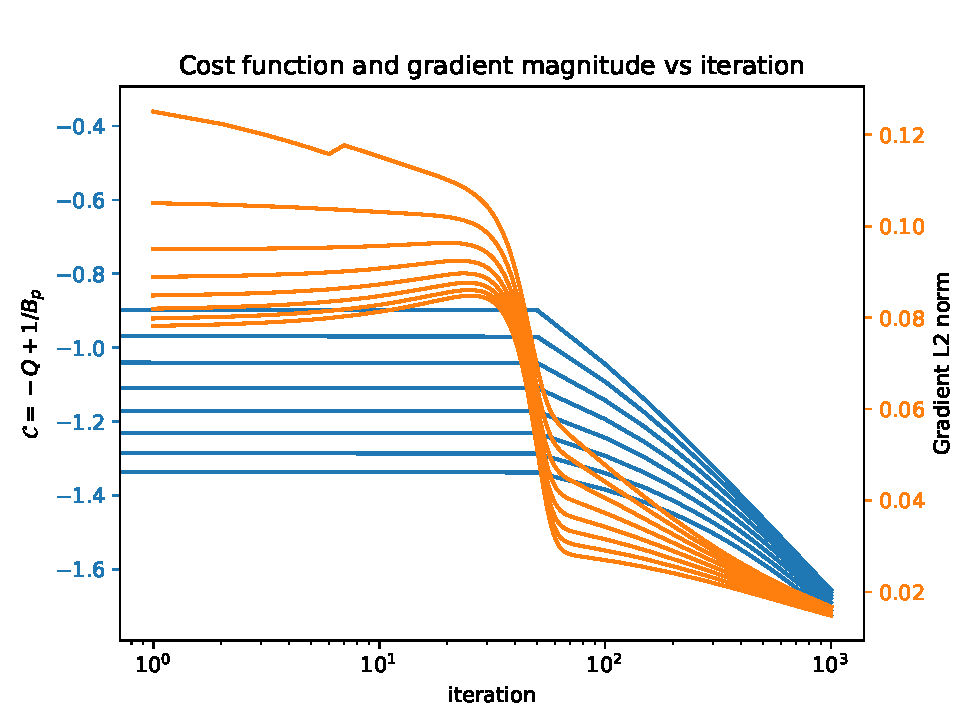
\includegraphics[scale=0.6]{opt_figures/simple_Q_cost_paper.pdf}
    \caption[Simple mirror: cost function and gradient magnitude for each step]{The cost function and gradient magnitude for each optimization step.}
    \label{fig:simple_Q_opt}
\end{figure}

\begin{figure}
    \centering
    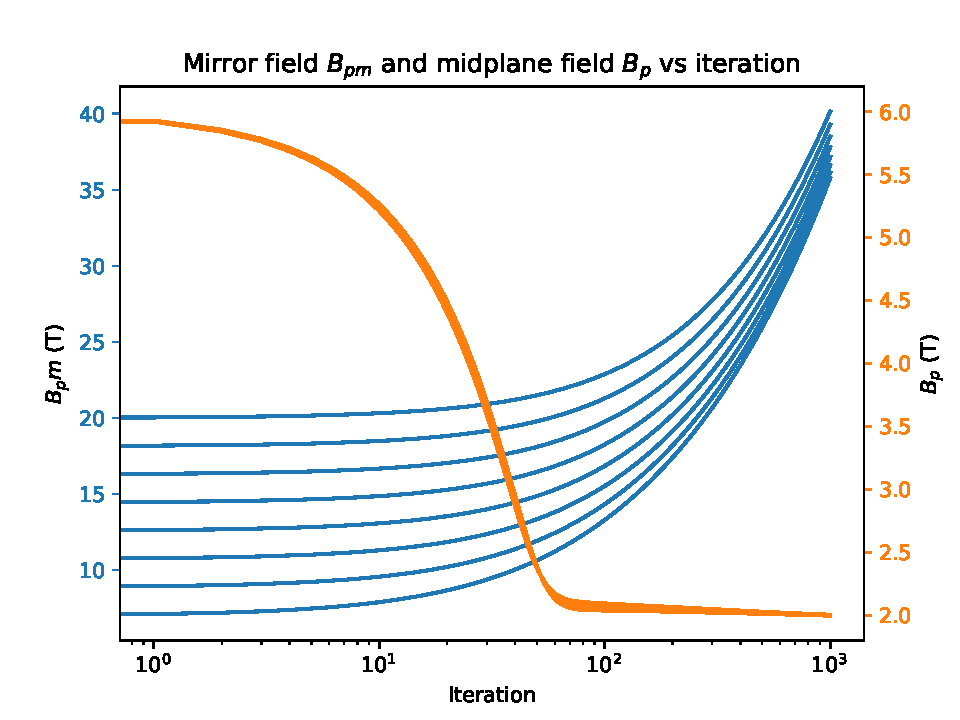
\includegraphics[scale=0.6]{opt_figures/mirror_field_iteration_paper.pdf}
    \caption[Simple mirror: magnetic fields for each step]{The mirror and midplane fields for each optimization step. Note the logarithmic x-axis — the rate of increase of the mirror field $B_{pm}$ with respect to optimization step decreases with iteration.}
    \label{fig:simple_Q_fields}
\end{figure}

\begin{figure}
    \centering
    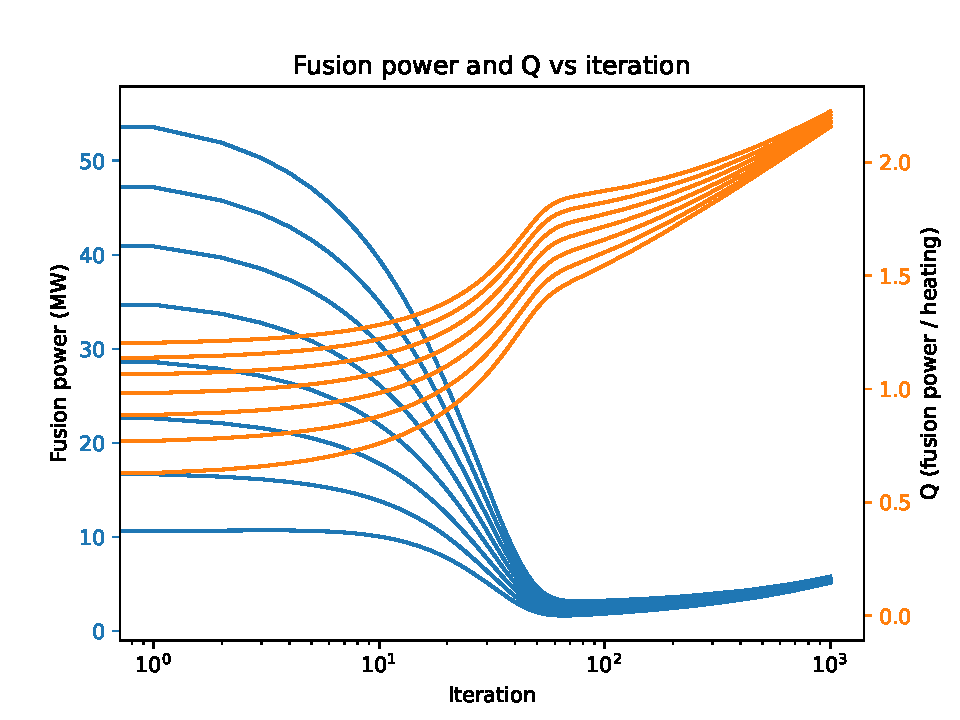
\includegraphics[scale=0.6]{opt_figures/Power_Q_vs_iteration_paper.pdf}
    \caption[Simple mirror: fusion power and Q for each step]{The total fusion power and Q for each optimizaiton step.}
    \label{fig:simple_Q_power}
\end{figure}

\begin{figure}
    \centering
    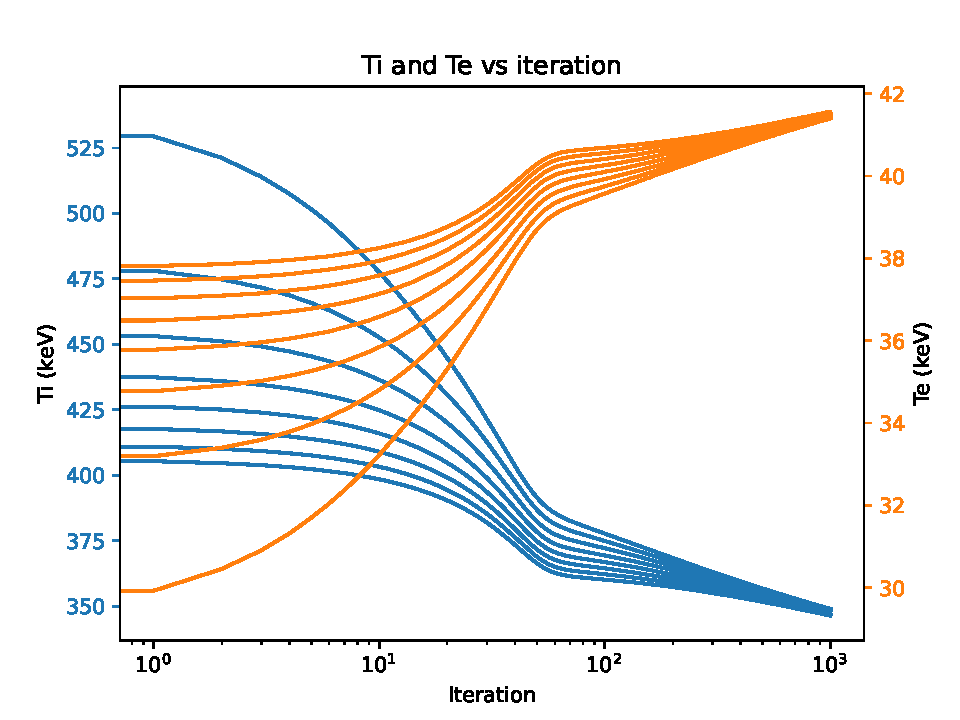
\includegraphics[scale=0.6]{opt_figures/Ti_Te_vs_iteration_paper.pdf}
    \caption[Simple mirror: temperatures for each step]{The ion and electron temperatures for each optimization step}
    \label{fig:simple_Q_temps}
\end{figure}

